In this section, we provide extended details in our experiment on setup and protocol, followed by visualization of more comprehensive results.
\subsection{Experiment details}
\label{subsec:app_exp_detail}
\begin{table}
	\caption{The configuration for Gaussian kernel and the search grid for initial learning rate on the Census, YearPred, Covtype and TIMIT datasets.}
	\label{tab:hyperparam}
	\begin{center}
	\begin{tabular}{lll}
	\toprule
	Dataset & $1/2\sigma^2$ & Learning rate grid \\
	\midrule
Census & 0.0006 & {0.01, 0.05, 0.1, \textbf{0.5}, 1.0} \\
YearPred & 0.01 & {0.05, 0.1, \textbf{0.5}, 1.0, 5.0} \\
Covtype & 0.6 & {1.0, 5.0, 10.0, \textbf{50.0}, 100.0} \\
TIMIT & 0.0015 & {5.0, 10.0, 50.0, \textbf{100.0}, 500.0} \\
	\bottomrule
	\end{tabular}
	\end{center}
	\label{tab:kernel_hyper}
\end{table}

\paragraph{Dataset details and kernel configuration}
In section~\ref{sec:experiments}, we demonstrate the performance of LP-RFFs on the TIMIT, YearPred, CovType and Census datasets, with SGD-based minibatch training. These datasets spans over regression, binary and multi-class classification tasks. We present the details, including task specification, dataset size and the number of raw data attributes in Table~\ref{tab:dataset_details}. In these experiments we use Gaussian kernel with the kernel width hyperparameter $\sigma$ recommended by~\cite{may2017} in Table~\ref{tab:kernel_hyper}. 
\begin{table}
	\caption{Dataset details.  For classification tasks, we write the number
		of classes in parentheses in the ``task'' column.}
	\label{tab:datasets}
%	\small
	\begin{center}
		\begin{tabular}{llllll} 
			\toprule
			\textbf{Dataset}  & \textbf{Task} & \textbf{Train} & \textbf{Heldout} & \textbf{Test} & \textbf{\#Attr.} \\ 
			\midrule
			CENSUS   & Reg.   & 16k   & 2k      & 2k   & 119 \\ 
			YEARPRED & Reg.   & 417k  & 46k     & 52k  & 90  \\ 
			COVTYPE  & Class. (2) & 418k  & 46k     & 116k & 54  \\ 
			TIMIT    & Class. (147) & 2.3M  & 245k    & 116k & 440 \\
			\bottomrule
		\end{tabular}
	\end{center}
	\label{tab:dataset_details}
\end{table}

\paragraph{Hyperparameter tuning for SGD-based training}
We use the heldout set in order to perform early stopping and determine when to decay the learning rate, as in \citep{morgan1990generalization,sainath2013b,sainath2013low}. Early stopping can be seen as a form of regularization \citep{zhang2005boosting,wei2017early}, and this saves us the effort of manually tuning the initial learning rate, the learning rate decay, the regularizer, and the number of training epochs.  The scheme works as follows: at the end of each epoch, we decay the learning rate in half if the heldout performance is less than $1\%$ better relative to the previous best model, using MSE for regression and cross entropy for classification. Furthermore, if the model performs \textit{worse} than the previous best, we revert the model. The training terminates after the learning rate has been decayed 10 times. Early stopping can be seen as a form of regularization \citep{zhang2005boosting,wei2017early}.  We use a single initial learning rate per dataset across all experiments, which we tune via grid search using $20\text{k}$ \Nystrom features. We choose to use \Nystrom features to tune the initial learning rate in order to avoid biasing the results in favor of RFF-based approaches.

\paragraph{Hyperparameter tuning for LM-HALP-based training}
We use the same learning rate schedule as the one in the SGD-based experiments. We sweep the $\mu$ parameter, which determines the value of the quantization scale in HALP, using grid search over $\{0.001, 0.01, 0.1, 1.0\}$. For each number of LP-RFFs $m$, we choose the value of $\mu$ attaining lowest heldout classification error, and report this as the error.

\subsection{Additional experiment results}
\label{subsec:app_additional_exp_res}
\paragraph{Empirical evaluations of LP-RFFs}
In Section~\ref{sec:full_run}, we demonstrate the generalization performance of LP-RFFs on the TIMIT and YearPred datasets. In this section, we demonstrate the full generalization performance comparison on the TIMIT, YearPred, CovType and Census datasets. In Figure~\ref{fig:generalization_col_app}, we show the generalization performance of 8, 4, 1 bit LP-RFFs, with FP-\Nystrom, FP-RFF and circulant FP-RFF as the full precision baselines. We can observe that LP-RFF, by using 4 or 8-bit quantized representation, can systematically outperform full precision baselines across the four datasets under different memory budgets.
%\begin{figure}
%	\centering
%	\begin{tabular}{@{\hskip 0in}c@{\hskip 0in}c@{\hskip 0in}c@{\hskip 0in}c@{\hskip 0in}}
%%		\subfigure[Census heldout MSE]{\label{fig:census_mem} 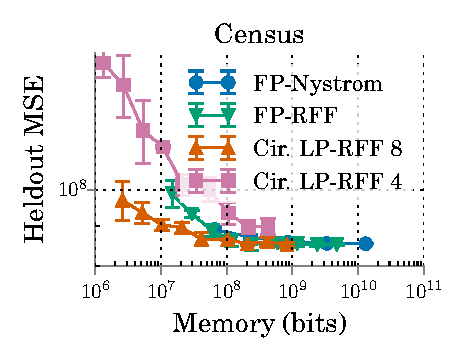
\includegraphics[width=0.3\linewidth]{figures/census_MSE_vs_n_memory.pdf} } \hfill
%%		\subfigure[Census heldout MSE]{\label{fig:census_feat}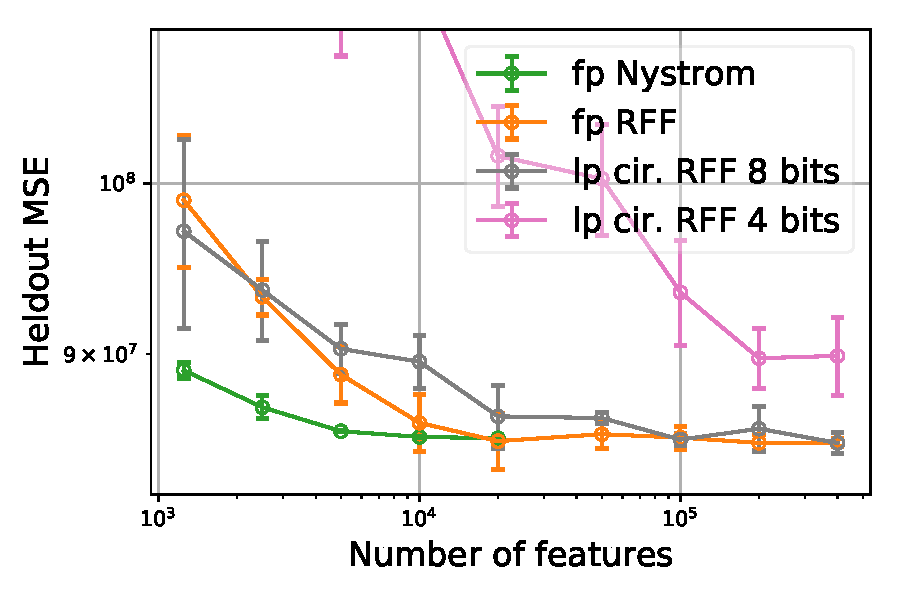
\includegraphics[width=0.3\linewidth]{figures/census_MSE_vs_n_feat.pdf} } \hfill
%%		\subfigure[CovType heldout error]{\label{fig:covtype_mem} 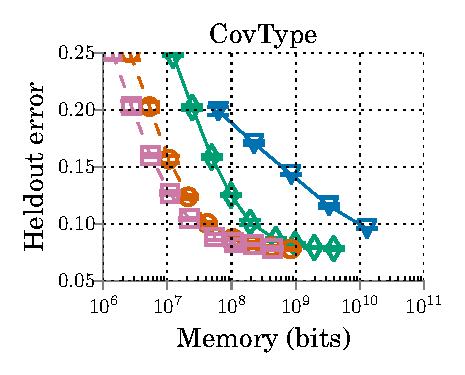
\includegraphics[width=0.3\linewidth]{figures/covtype_error_vs_n_memory.pdf} } \hfill
%%		\subfigure[CovType heldout error]{\label{fig:covtype_feat}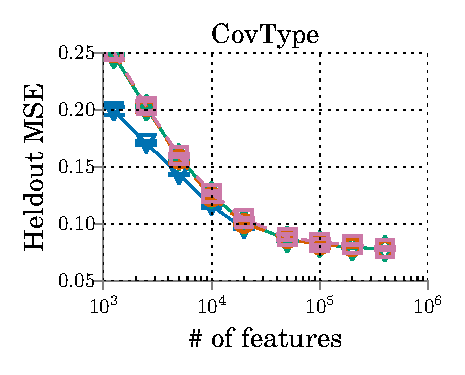
\includegraphics[width=0.3\linewidth]{figures/covtype_error_vs_n_feat.pdf} } \hfill
%%		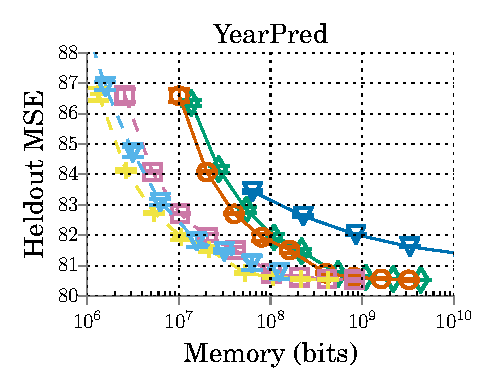
\includegraphics[width=0.3\linewidth]{figures/yearpred_MSE_vs_n_memory_all_line.pdf} &
%%		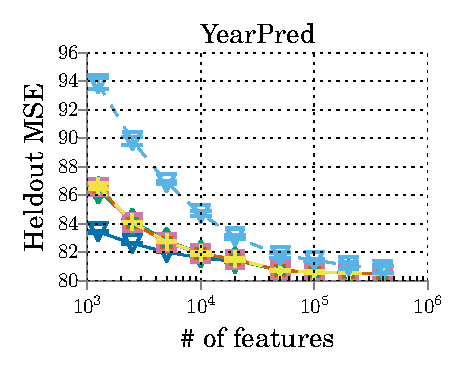
\includegraphics[width=0.3\linewidth]{figures/yearpred_MSE_vs_n_feat_all_line.pdf} &
%%		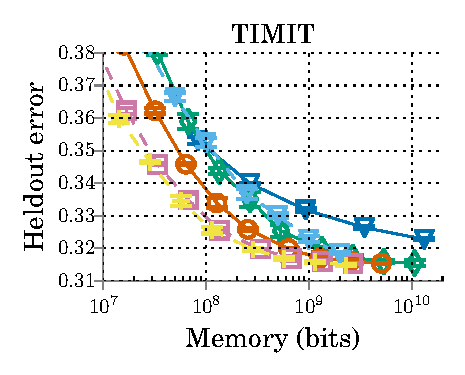
\includegraphics[width=0.3\linewidth]{figures/timit_error_vs_n_memory_all_line.pdf} &
%%		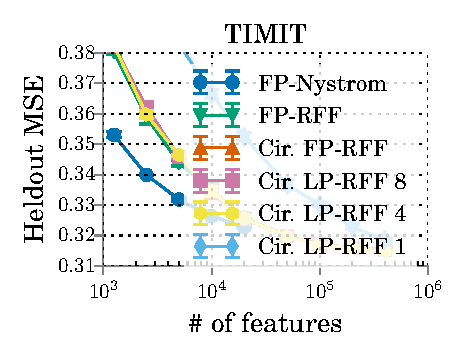
\includegraphics[width=0.3\linewidth]{figures/timit_error_vs_n_feat_all_line.pdf} \\
%%		(a) Census & (b) YearPred & (c) Covtype & (d) TIMIT \\
%		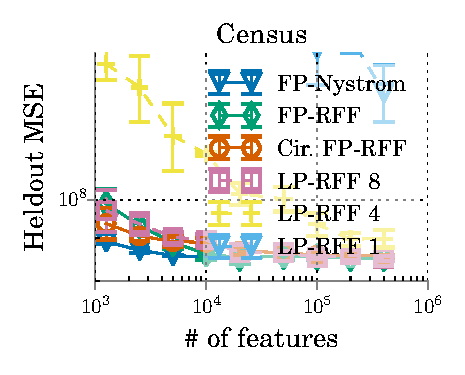
\includegraphics[width=0.26\linewidth]{figures/census_MSE_vs_n_feat_all_line.pdf} &
%		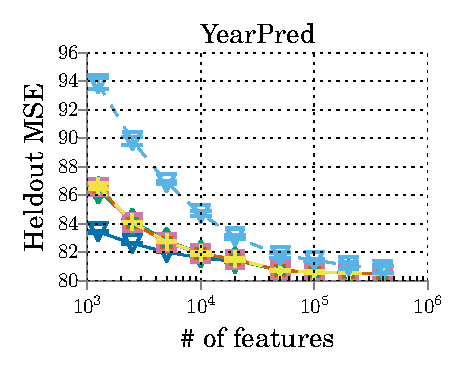
\includegraphics[width=0.26\linewidth]{figures/yearpred_MSE_vs_n_feat_all_line.pdf} &
%		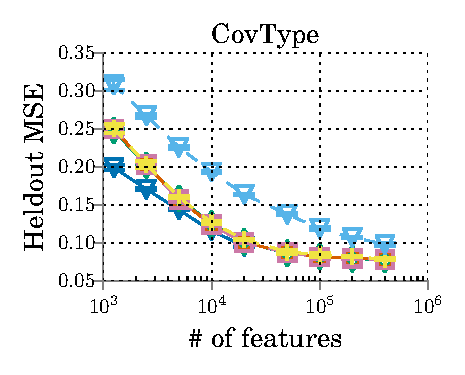
\includegraphics[width=0.26\linewidth]{figures/covtype_error_vs_n_feat_all_line.pdf} &
%		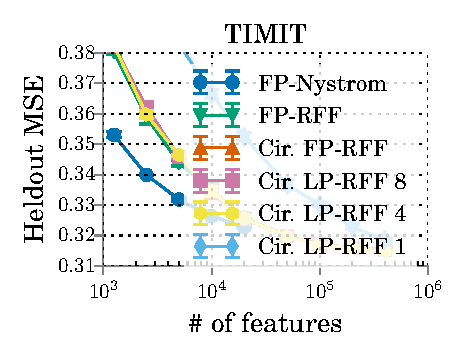
\includegraphics[width=0.26\linewidth]{figures/timit_error_vs_n_feat_all_line.pdf} \\
%		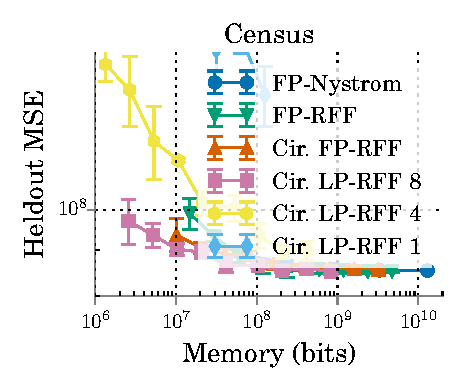
\includegraphics[width=0.26\linewidth]{figures/census_MSE_vs_n_memory_all_line.pdf} &
%		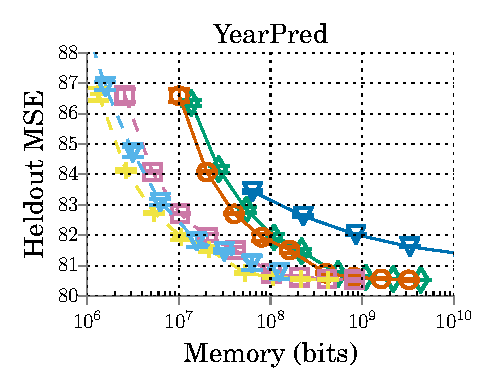
\includegraphics[width=0.26\linewidth]{figures/yearpred_MSE_vs_n_memory_all_line.pdf} &
%		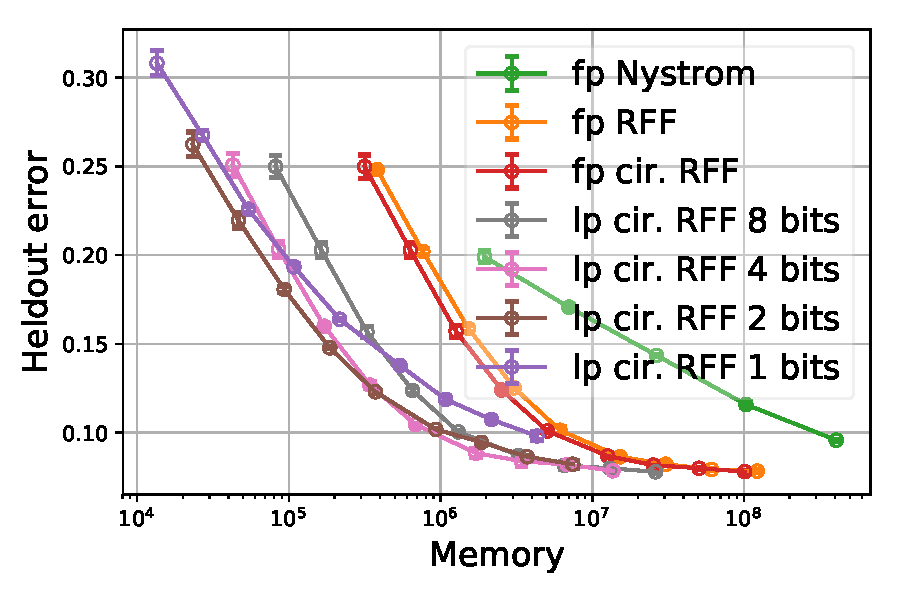
\includegraphics[width=0.26\linewidth]{figures/covtype_error_vs_n_memory_all_line.pdf} &
%		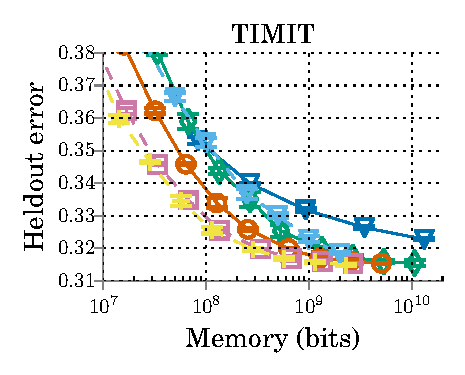
\includegraphics[width=0.26\linewidth]{figures/timit_error_vs_n_memory_all_line.pdf} \\
%%		(a) Census & (b) YearPred & (c) Covtype & (d) TIMIT \\
%	\end{tabular}
%	\caption{Generalization performance of LP RFF, full precision RFF and \Nystrom with respect to number of features and memory budgets. We can observe that LP RFFs demonstrate better generalization performance than full precision baselines under memory budget. Noticeably, the comparison of different methods on generalization performance behaves differently under memory budget and under number off features. E.g., \Nystrom shows better generalization performance than RFF based approach with the same number of features. However, \Nystrom can be significantly worse under memory budgets.}
%	\label{fig:generalization_col_app}
%\end{figure}
\begin{figure}
	\centering
	\vspace{-4em}
	\begin{tabular}{c c}
%	\begin{tabular}{@{\hskip -0.1in}c@{\hskip 0.0in}c@{\hskip -0.1in}}
%		\subfigure[Census heldout MSE]{\label{fig:census_mem} 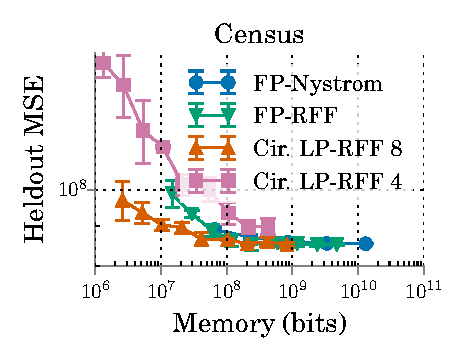
\includegraphics[width=0.3\linewidth]{figures/census_MSE_vs_n_memory.pdf} } \hfill
%		\subfigure[Census heldout MSE]{\label{fig:census_feat}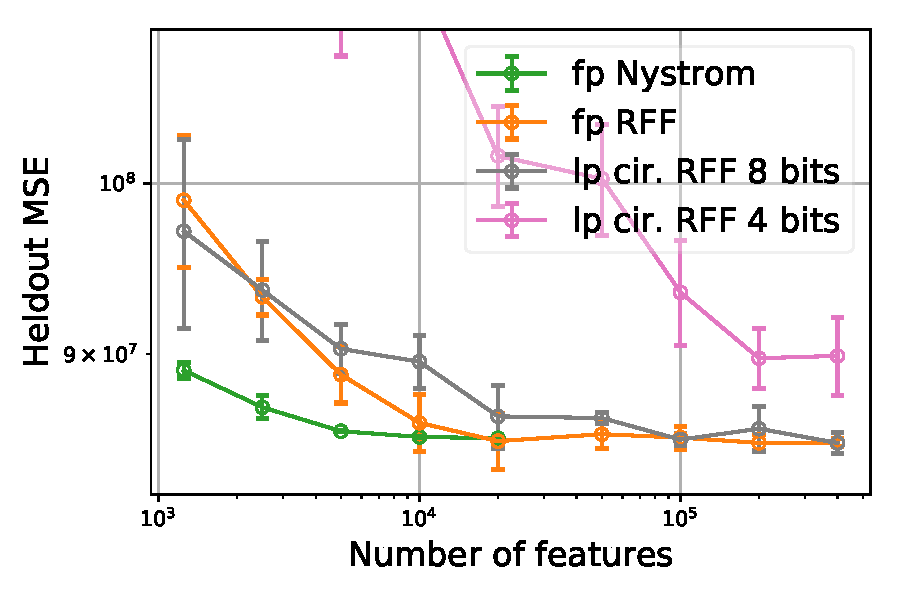
\includegraphics[width=0.3\linewidth]{figures/census_MSE_vs_n_feat.pdf} } \hfill
%		\subfigure[CovType heldout error]{\label{fig:covtype_mem} 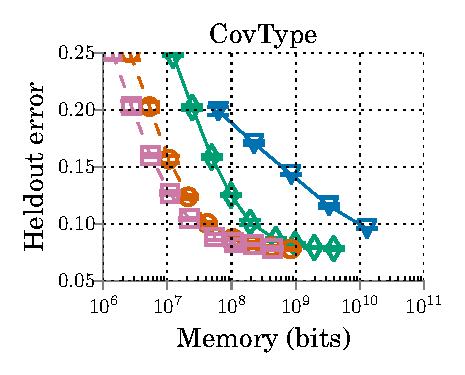
\includegraphics[width=0.3\linewidth]{figures/covtype_error_vs_n_memory.pdf} } \hfill
%		\subfigure[CovType heldout error]{\label{fig:covtype_feat}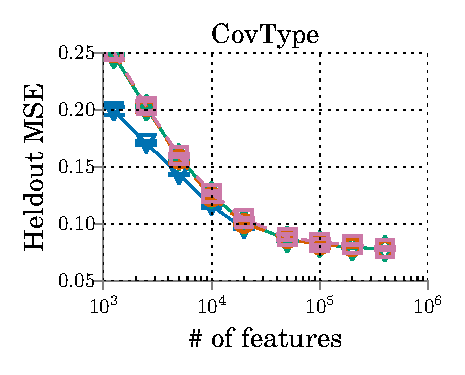
\includegraphics[width=0.3\linewidth]{figures/covtype_error_vs_n_feat.pdf} } \hfill
%		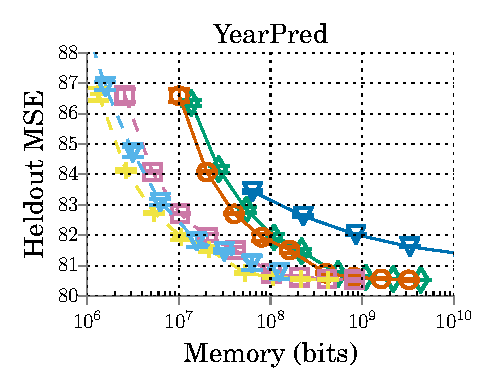
\includegraphics[width=0.3\linewidth]{figures/yearpred_MSE_vs_n_memory_all_line.pdf} &
%		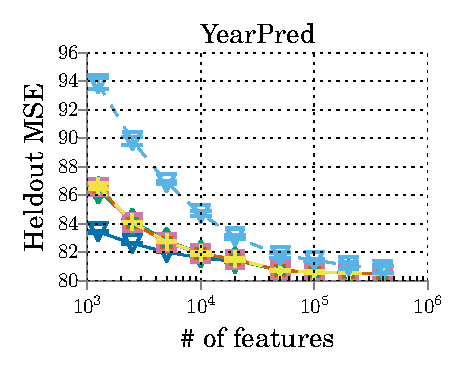
\includegraphics[width=0.3\linewidth]{figures/yearpred_MSE_vs_n_feat_all_line.pdf} &
%		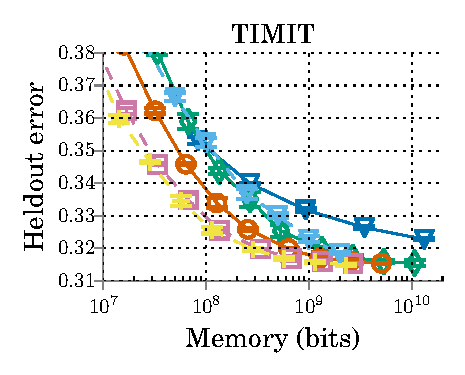
\includegraphics[width=0.3\linewidth]{figures/timit_error_vs_n_memory_all_line.pdf} &
%		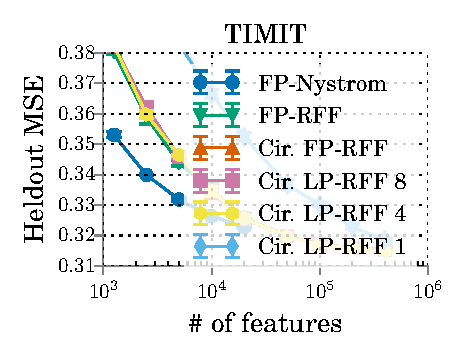
\includegraphics[width=0.3\linewidth]{figures/timit_error_vs_n_feat_all_line.pdf} \\
%		(a) Census & (b) YearPred & (c) Covtype & (d) TIMIT \\

%		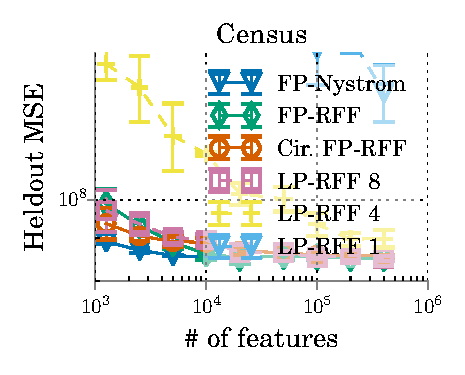
\includegraphics[width=0.4\linewidth]{figures/census_MSE_vs_n_feat_all_line.pdf} &
%		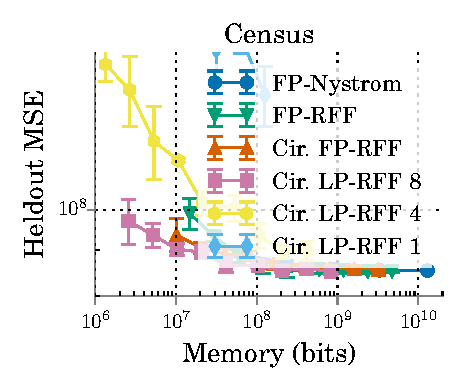
\includegraphics[width=0.4\linewidth]{figures/census_MSE_vs_n_memory_all_line.pdf} \\
%		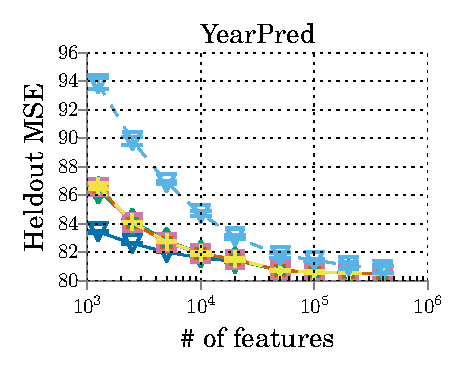
\includegraphics[width=0.4\linewidth]{figures/yearpred_MSE_vs_n_feat_all_line.pdf} &
%		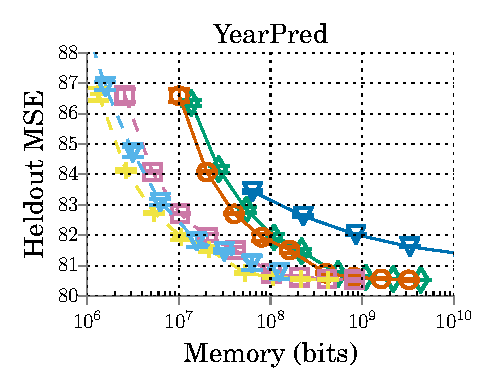
\includegraphics[width=0.4\linewidth]{figures/yearpred_MSE_vs_n_memory_all_line.pdf} \\
%		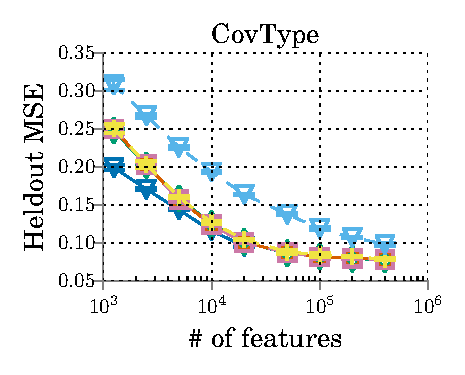
\includegraphics[width=0.4\linewidth]{figures/covtype_error_vs_n_feat_all_line.pdf} &
%		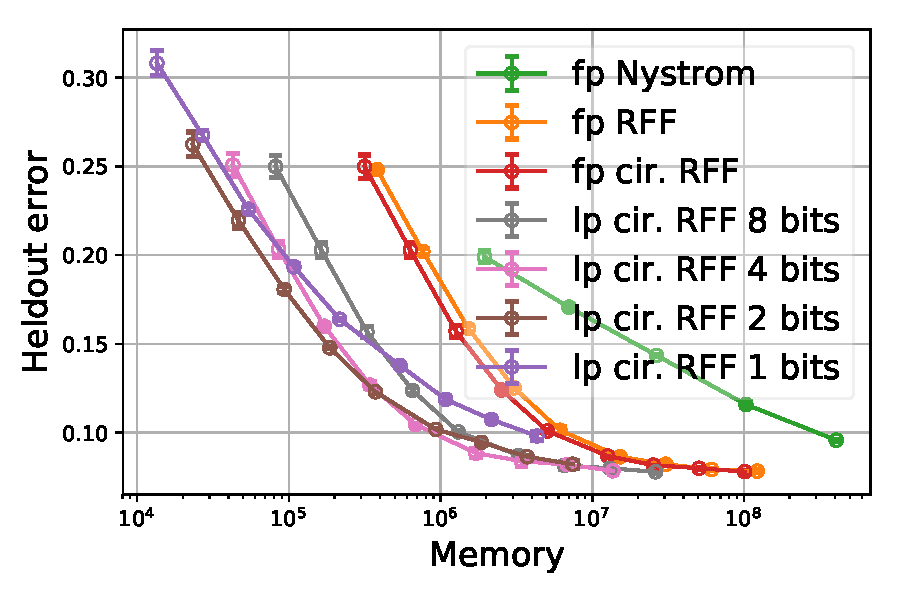
\includegraphics[width=0.4\linewidth]{figures/covtype_error_vs_n_memory_all_line.pdf} \\
%		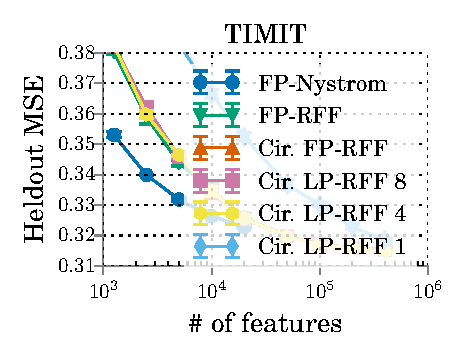
\includegraphics[width=0.4\linewidth]{figures/timit_error_vs_n_feat_all_line.pdf} &
%		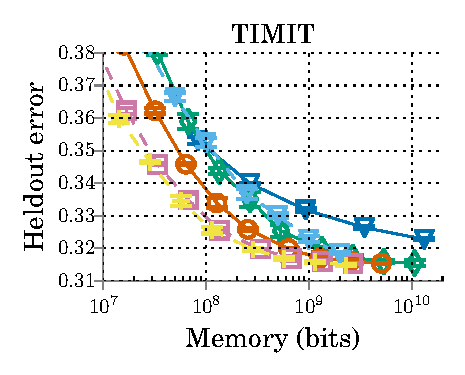
\includegraphics[width=0.4\linewidth]{figures/timit_error_vs_n_memory_all_line.pdf} \\
%		(a) Census & (b) YearPred & (c) Covtype & (d) TIMIT \\
		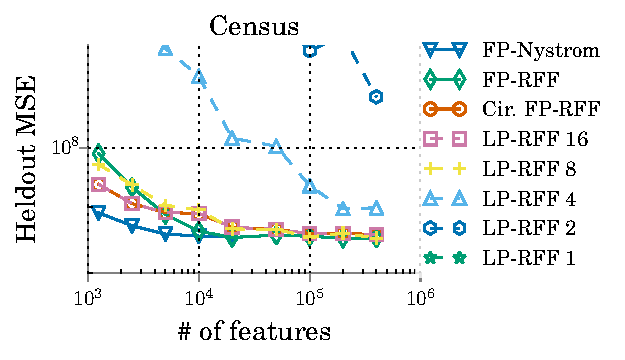
\includegraphics[height=0.3\linewidth]{figures/census_MSE_vs_n_feat_every_line.pdf} &
		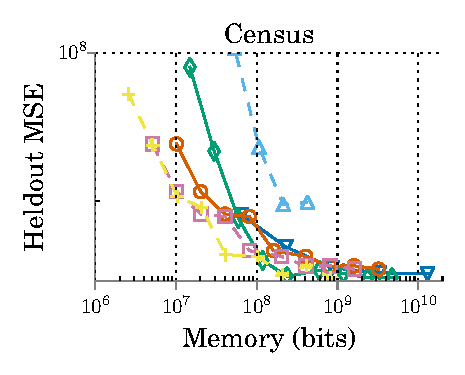
\includegraphics[height=0.3\linewidth]{figures/census_MSE_vs_n_memory_every_line.pdf} \\ [-0.5em]
		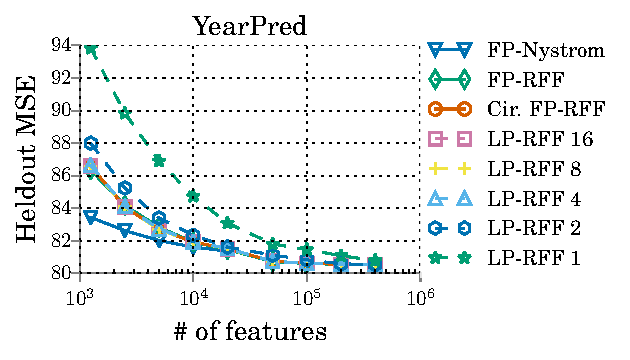
\includegraphics[height=0.3\linewidth]{figures/yearpred_MSE_vs_n_feat_every_line.pdf} &
		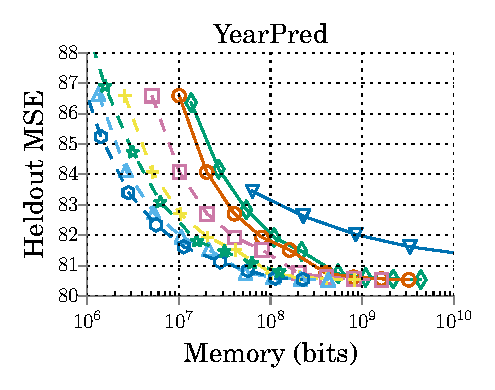
\includegraphics[height=0.3\linewidth]{figures/yearpred_MSE_vs_n_memory_every_line.pdf} \\ [-0.5em]
		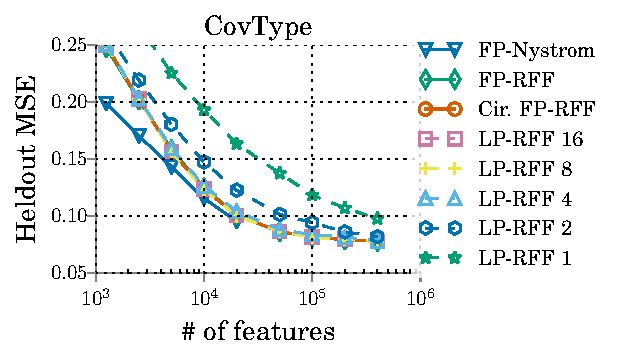
\includegraphics[height=0.3\linewidth]{figures/covtype_error_vs_n_feat_every_line.pdf} &
		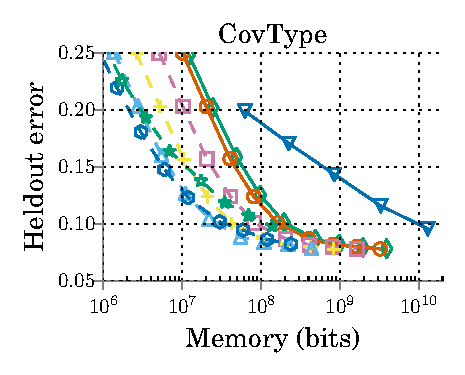
\includegraphics[height=0.3\linewidth]{figures/covtype_error_vs_n_memory_every_line.pdf} \\ [-0.5em]
		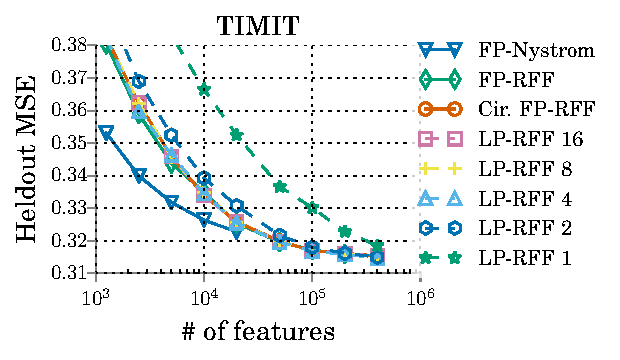
\includegraphics[height=0.3\linewidth]{figures/timit_error_vs_n_feat_every_line.pdf} &
		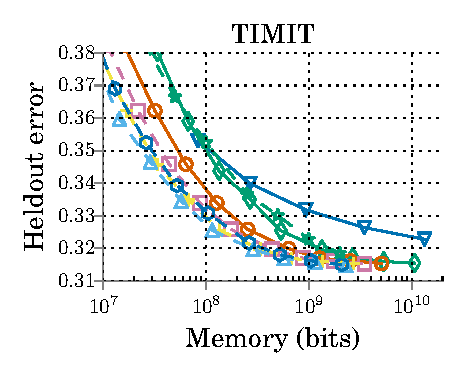
\includegraphics[height=0.3\linewidth]{figures/timit_error_vs_n_memory_every_line.pdf} \\ [-1em]
	\end{tabular}
	\caption{Generalization performance of LP RFF, full precision RFF and \Nystrom with respect to number of features and memory budgets. We can observe that LP RFFs demonstrate better generalization performance than full precision baselines under memory budget. Noticeably, the comparison of different methods on generalization performance behaves differently under memory budget and under number off features. E.g., \Nystrom shows better generalization performance than RFF based approach with the same number of features. However, \Nystrom can be significantly worse under memory budgets. Additional, we observe 8, 4 or 2 bits LP-RFFs is typically the best performing approach on the four datasets.}
	\label{fig:generalization_col_app}
\end{figure}

\paragraph{Generalization performance vs. relative spectral distance}
In Section~\ref{subsec:perf_vs_rel_spec_dist}, we empirically demonstrate correlation between generalization performance and relative spectral distance. To give an extended view on the correlation, we demonstrate full results on 8, 4, 1-bits LP-RFFs, together with the full precision baselines in Figure~\ref{fig:specdist_app}. In Figure~\ref{fig:specdist_app} (left), we can observe, on both the Census and CovType datasets, relative spectral distance can be predictive for the performance across different methods; i.e. similar relative spectral distance can imply similar generalization performance across different methods. In the contrast, \Nystrom and RFF based approaches can demonstrate significantly different spectral norm and Frobenius norm of $K - \tilde{K}$, the difference of the exact kernel matrix and its approximation.

\paragraph{Low precision training using low-precision LM-Bit-Center SGD}
To enable the computational benefits of LP-RFFs on real systems, we investigate low-precision training using LM-HALP~\cite{halp18} for linear models in Section~\ref{sec:halp}. During the iterative model update steps, LM-HALP use a technique called \textbf{bit-centering} to reparameterize the linear model using low-precision fixed-point representations. This allows all the matrix multiplication involved in stochastic model updates using integer operations on fixed-point representation.
	LM-HALP reduces memory footprint by using low-precision fixed-point model parameterization during the iterative model updates. However, LM-HALP needs to store the full-dataset gradient (which is periodically computed) in low-precision fixed-point representation during the model updates. To further eliminate this additional memory consumption, we preliminarily experiment with low precision training using LM-Bit-Center SGD, a straight-forward variant of LM-HALP. LM-Bit-Center SGD is the same as LM-HALP, except using simple SGD updates instead of SVRG updates; in this way, LM-Bit-Center SGD don't need to keep the full-dataset gradient (in low-precision fixed-point representation) during model update steps. Specifically in our experiments, we run 8-bit LM-Bit-Center SGD on 8-bit LP-RFFs for the TIMIT dataset. As shown in Figure~\ref{fig:lm_bit_center}, when the number of features is at least 10000, we can observe that the heldout error from low-precision 8-bit LM-Bit-Center SGD closely matches the ones from full-precision SGD and low-precision 8-bit LM-HALP training.

\begin{figure}
\centering
%	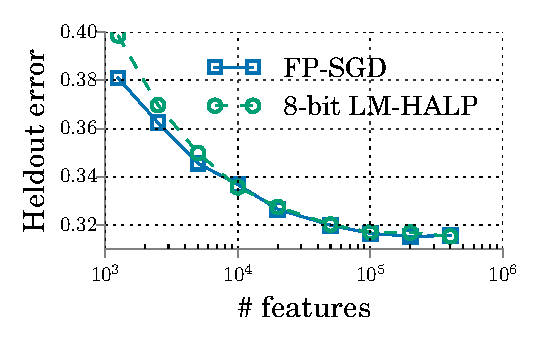
\includegraphics[width=0.975\linewidth]{figures/timit_error_vs_n_feat_lm_halp.pdf}
	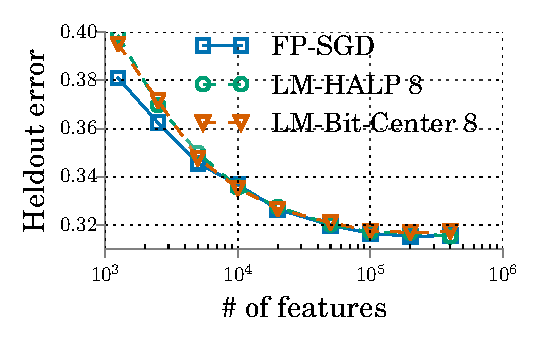
\includegraphics[width=0.4\linewidth]{figures/timit_error_vs_n_feat_lm_bit_center_sgd.pdf}
%	\caption{Low-precision training on TIMIT using 8-bit LM-HALP on 8-bit LP-RFFs, relative to full-precision SGD.
%		%Low precision training with HALP can demonstrate similar generalization performance as full precision training with SGD.
%	}	
	\caption{Low-precision 8-bit LM-HALP, 8-bit LM-Bit-Center-SGD and full-precision SGD training with 8-bit LP-RFFs for TIMIT.}	
	\label{fig:lm_bit_center}
\end{figure}


\begin{figure}
	\centering
	\vspace{-4em}
	\begin{tabular}{c c}
%	\begin{tabular}{@{\hskip -0.15in}c@{\hskip -0.15in}c@{\hskip -0.15in}}
		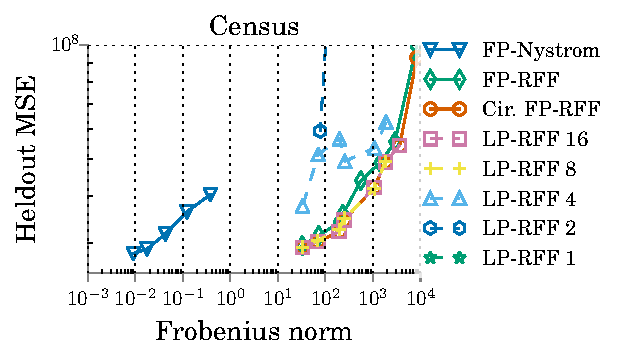
\includegraphics[height=0.3\linewidth]{figures/regression_l2_vs_f_norm_every_line.pdf} &
		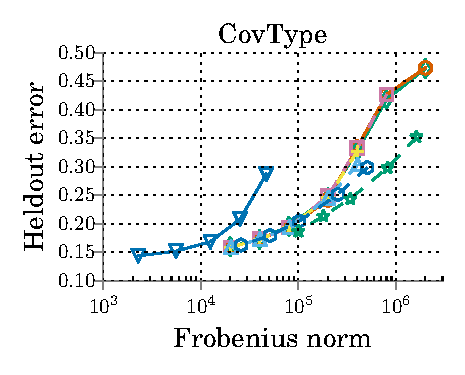
\includegraphics[height=0.3\linewidth]{figures/classification_acc_vs_f_norm_every_line.pdf} \\
		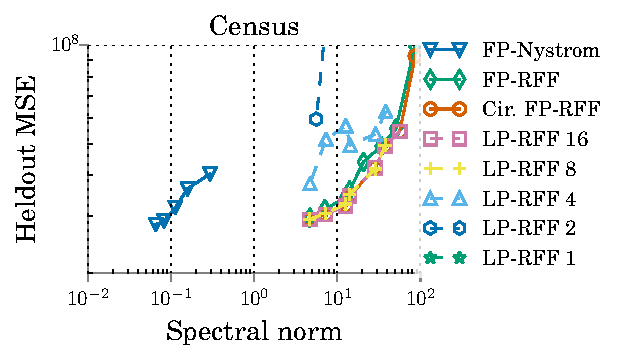
\includegraphics[height=0.3\linewidth]{figures/regression_l2_vs_s_norm_every_line.pdf} &
		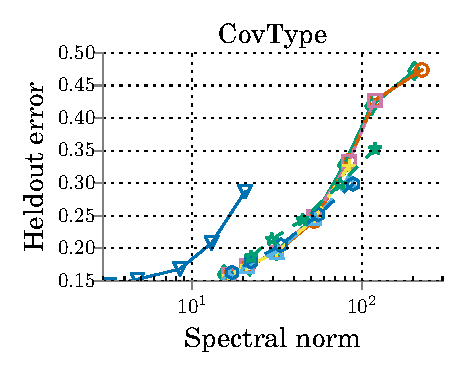
\includegraphics[height=0.3\linewidth]{figures/classification_acc_vs_s_norm_every_line.pdf} \\
		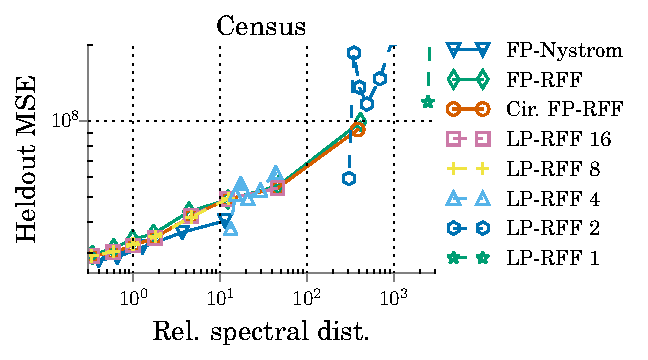
\includegraphics[height=0.3\linewidth]{figures/regression_l2_vs_delta_every_line.pdf} &
		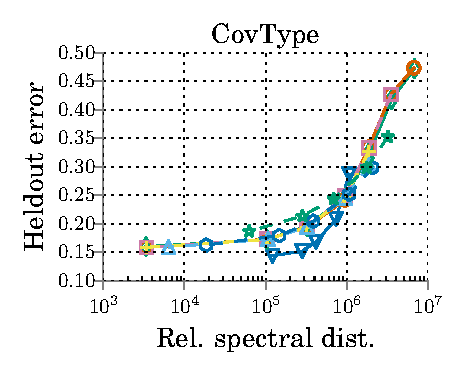
\includegraphics[height=0.3\linewidth]{figures/classification_acc_vs_delta_every_line.pdf} \\
		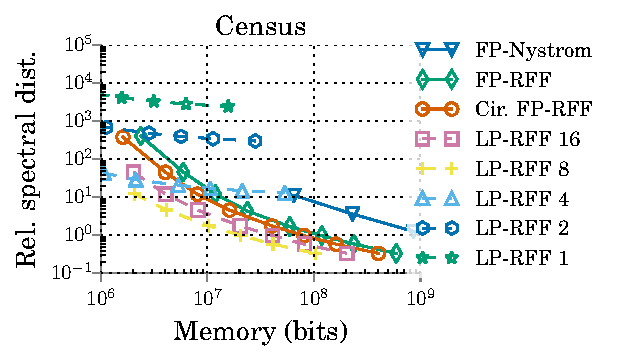
\includegraphics[height=0.3\linewidth]{figures/regression_delta_vs_mem_every_line.pdf} &
		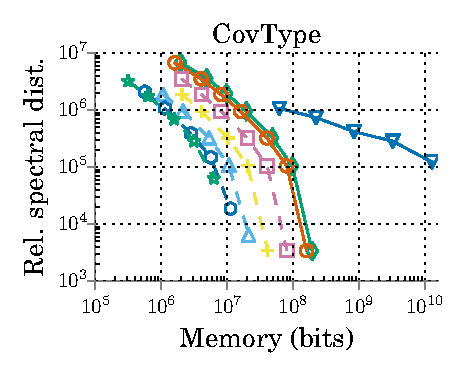
\includegraphics[height=0.3\linewidth]{figures/classification_delta_vs_mem_every_line.pdf} \\
	\end{tabular}
%	\begin{tabular}{@{\hskip -0.25in}c@{\hskip -0.25in}c@{\hskip -0.25in}c@{\hskip -0.25in}}
%		\subfigure[MSE and Rel. spectral distance distance]{\label{fig:census_delta_all_line} \includegraphics[width=0.33\linewidth]{figures/regression_l2_vs_delta_all_line.pdf} } \hfill
%		\subfigure[MSE and Frobenius norm]{\label{fig:census_f_norm_all_line} \includegraphics[width=0.33\linewidth]{figures/regression_l2_vs_f_norm_all_line.pdf} } \hfill
%		\subfigure[Rel. spectral distance distance and memory]{\label{fig:census_s_norm_all_line}  \includegraphics[width=0.33\linewidth]{figures/regression_l2_vs_s_norm_all_line.pdf} } \hfill \\
%		\subfigure[MSE and Frobenius norm]{\label{fig:covtype_delta_all_line} \includegraphics[width=0.33\linewidth]{figures/classification_acc_vs_delta_all_line.pdf} } \hfill
%		\subfigure[Error and Frobenius norm]{\label{fig:covtype_f_norm_all_line} \includegraphics[width=0.33\linewidth]{figures/classification_acc_vs_f_norm_all_line.pdf} } \hfill
%		\subfigure[Error and spectral norm]{\label{fig:covtype_s_norm_all_line} \includegraphics[width=0.33\linewidth]{figures/classification_acc_vs_s_norm_all_line.pdf}} \hfill
%	\end{tabular}
	\caption{Generalization performance vs. relative spectral distance $D_{\lambda}(K,\tK)$, the Frobenius and spectral norms of $K - \tK$. We observe that $D_{\lambda}(K,\tK)$ aligns much better with generalization performance than the Frobenius and spectral norms, for both the Census and sub-sampled CovType datasets. Under memory budgets, we can also observe (in the last row of the figures) that approximation method with better generalization performance also demonstrate low relative spectral distances.}
	\label{fig:specdist_app}	
%	\begin{tabular}{c c c}
%		\includegraphics[width=0.33\linewidth]{figures/regression_delta_vs_mem_all_line.pdf} &
%		\includegraphics[width=0.33\linewidth]{figures/regression_l2_vs_mem_all_line.pdf} &
%		\includegraphics[width=0.33\linewidth]{figures/regression_l2_vs_delta_all_line.pdf} \\
%		\includegraphics[width=0.33\linewidth]{figures/classification_delta_vs_mem_all_line.pdf} &
%		\includegraphics[width=0.33\linewidth]{figures/classification_acc_vs_mem_all_line.pdf} &
%		\includegraphics[width=0.33\linewidth]{figures/classification_acc_vs_delta_all_line.pdf} \\
%		(a) & (b) & (c)
%	\end{tabular}
%	\caption{The strong correlation between generalization performance and $\lambda$-spectral distance $D_{\lambda}(K,\tK)$ under memory budgets for the Census dataset (top) and subsampled CovType dataset (bottom). Under different memory budget in (a) and (b), the precision demonstrates smaller $D_{\lambda}(K,\tK)$ tends to have better generalization performance. In (c), different kernel approximation approaches demonstrate similar generalization performance for similar $\lambda$-spectral distance.}
%	\label{fig:specdist_app}
\end{figure}



%\begin{figure}
%	\centering
%	\begin{tabular}{@{\hskip -0.25in}c@{\hskip -0.25in}c@{\hskip -0.25in}c@{\hskip -0.25in}}
%		\includegraphics[width=0.33\linewidth]{figures/regression_l2_vs_delta_all_line.pdf} &
%		\includegraphics[width=0.33\linewidth]{figures/regression_l2_vs_f_norm_all_line.pdf} &
%		\includegraphics[width=0.33\linewidth]{figures/regression_l2_vs_s_norm_all_line.pdf} \\
%		\includegraphics[width=0.33\linewidth]{figures/classification_acc_vs_delta_all_line.pdf} &
%		\includegraphics[width=0.33\linewidth]{figures/classification_acc_vs_f_norm_all_line.pdf} &
%		\includegraphics[width=0.33\linewidth]{figures/classification_acc_vs_s_norm_all_line.pdf} \\
%	\end{tabular}
%%	\begin{tabular}{@{\hskip -0.25in}c@{\hskip -0.25in}c@{\hskip -0.25in}c@{\hskip -0.25in}}
%%		\subfigure[MSE and Rel. spectral distance distance]{\label{fig:census_delta_all_line} \includegraphics[width=0.33\linewidth]{figures/regression_l2_vs_delta_all_line.pdf} } \hfill
%%		\subfigure[MSE and Frobenius norm]{\label{fig:census_f_norm_all_line} \includegraphics[width=0.33\linewidth]{figures/regression_l2_vs_f_norm_all_line.pdf} } \hfill
%%		\subfigure[Rel. spectral distance distance and memory]{\label{fig:census_s_norm_all_line}  \includegraphics[width=0.33\linewidth]{figures/regression_l2_vs_s_norm_all_line.pdf} } \hfill \\
%%		\subfigure[MSE and Frobenius norm]{\label{fig:covtype_delta_all_line} \includegraphics[width=0.33\linewidth]{figures/classification_acc_vs_delta_all_line.pdf} } \hfill
%%		\subfigure[Error and Frobenius norm]{\label{fig:covtype_f_norm_all_line} \includegraphics[width=0.33\linewidth]{figures/classification_acc_vs_f_norm_all_line.pdf} } \hfill
%%		\subfigure[Error and spectral norm]{\label{fig:covtype_s_norm_all_line} \includegraphics[width=0.33\linewidth]{figures/classification_acc_vs_s_norm_all_line.pdf}} \hfill
%%	\end{tabular}
%	\caption{Generalization performance vs. relative spectral distance $D_{\lambda}(K,\tK)$, and that Frobenius and spectral norms of $K - \tK$. We observe that $D_{\lambda}(K,\tK)$ aligns much better with generalization performance than the Frobenius and spectral norms, for both the Census and sub-sampled CovType datasets.}
%	\label{fig:specdist_app}	
%%	\begin{tabular}{c c c}
%%		\includegraphics[width=0.33\linewidth]{figures/regression_delta_vs_mem_all_line.pdf} &
%%		\includegraphics[width=0.33\linewidth]{figures/regression_l2_vs_mem_all_line.pdf} &
%%		\includegraphics[width=0.33\linewidth]{figures/regression_l2_vs_delta_all_line.pdf} \\
%%		\includegraphics[width=0.33\linewidth]{figures/classification_delta_vs_mem_all_line.pdf} &
%%		\includegraphics[width=0.33\linewidth]{figures/classification_acc_vs_mem_all_line.pdf} &
%%		\includegraphics[width=0.33\linewidth]{figures/classification_acc_vs_delta_all_line.pdf} \\
%%		(a) & (b) & (c)
%%	\end{tabular}
%%	\caption{The strong correlation between generalization performance and $\lambda$-spectral distance $D_{\lambda}(K,\tK)$ under memory budgets for the Census dataset (top) and subsampled CovType dataset (bottom). Under different memory budget in (a) and (b), the precision demonstrates smaller $D_{\lambda}(K,\tK)$ tends to have better generalization performance. In (c), different kernel approximation approaches demonstrate similar generalization performance for similar $\lambda$-spectral distance.}
%%	\label{fig:specdist_app}
%\end{figure}

\subsection{Low-precision \Nystrom}
\label{sec:lpnystrom}
\begin{figure}
\centering
\begin{tabular}{c c}
	\includegraphics[width=0.4\linewidth]{figures/lp_nystrom_mse_vs_mem.pdf} &
	\includegraphics[width=0.4\linewidth]{figures/lp_ensemble_nystrom_mse_vs_mem.pdf} \\
	\includegraphics[width=0.4\linewidth]{figures/lp_nystrom_delta_vs_mem.pdf} &
	\includegraphics[width=0.4\linewidth]{figures/lp_ensemble_nystrom_delta_vs_mem.pdf} \\
	(a) LP-\Nystrom & (b) Ensemble LP-\Nystrom
\end{tabular}
\caption{The generalization performance and relative spectral distance of Low-precision \Nystrom and low-precision ensemble \Nystrom.}	
\end{figure}

For our initial experiments, we applied the same stochastic quantization to \Nystrom as to RFFs on the Census dataset. For both LP-\Nystrom and ensemble \Nystrom with 10 blocks~\cite{ensemble09}, we determine the quantization dynamic range with the maximum and minimum value from the \Nystrom features generated from training set. Due to the large dynamic range, we observe for LP-\NystromNS, the generalization performance degrades significant with less than or equal to 8 bits compared to full-precision \NystromNS. We reduce the dynamic range by a factor of $\sqrt{r}$ with $r$ learners using ensemble \NystromNS. Ensemble \Nystrom has the additional benefits on reducing the memory requirement in generating \Nystrom features. However, we observe ensemble \Nystrom demonstrates larger relative spectral distance compared to FP-\Nystrom, which aligns with its degraded empirical heldout MSE.




